\documentclass[12pt]{article}

\usepackage{isabelle}
\usepackage{isabellesym}

% this should be the last package used
\usepackage{pdfsetup}

\usepackage{amsmath}
\usepackage{graphicx}

% urls in roman style, theory text in math-similar italics
\urlstyle{rm}
\isabellestyle{it}

% sane default for proof documents
\parindent 0pt\parskip 0.5ex

\begin{document}

\title{Consensus Refined}
\begin{abstract}
  Algorithms for solving the consensus problem are fundamental to
  distributed computing. Despite their brevity, their
  ability to operate in concurrent, asynchronous and failure-prone
  environments comes at the cost of complex and subtle
  behaviors. Accordingly, understanding how they work and proving
  their correctness is a non-trivial endeavor where abstraction
  is immensely helpful.
%  
  Moreover, research on consensus has yielded a large number of
  algorithms, many of which appear to share common algorithmic
  ideas. A natural question is whether and how these similarities can
  be distilled and described in a precise, unified 
  way.
%
  In this work, we combine stepwise refinement and
  lockstep models to provide an abstract and unified
  view of a sizeable family of consensus algorithms. Our models
  provide insights into the design choices underlying the different 
  algorithms, and classify them based on those choices.  
\end{abstract}

\maketitle
\tableofcontents

\newpage

\section{Introduction}
\label{sec:introduction}

\emph{Distributed consensus} is a fundamental problem in distributed
computing: a fixed set of processes must \textit{agree} on a single
value from a set of proposed ones. Algorithms that solve this problem
provide building blocks for many higher-level tasks, such as
distributed leases, group membership, atomic broadcast (also known as
total-order broadcast or multi-consensus), and so forth. These in turn
provide building blocks for yet higher-level tasks like system
replication. In this work, however, our focus is on consensus
algorithms ``proper'', rather than their applications.
Namely, we consider consensus algorithms for the asynchronous
message-passing setting with benign link and process failures. 

Although the setting we consider explicitly excludes malicious
behavior, the interplay of concurrency, asynchrony, and failures can
still drive the execution of any consensus algorithm in many different
ways. This makes the understanding of both the algorithms and their
correctness non-trivial. Furthermore, many consensus algorithms have
been proposed in the literature. Many of these algorithms appear to
share similar underlying algorithmic ideas, although their
presentation, structure and details differ. A natural question is
whether these similarities can be distilled and captured in a uniform
and generic way. In the same vein, one may ask whether the algorithms
can be classified by some natural criteria.

This formalization, which accompanies our conference
paper~\cite{maric_consensus_15}, is our contribution towards
addressing these issues. Our primary tool in tackling them is
\emph{abstraction}. We describe consensus algorithms using
\emph{stepwise refinement}. In this method, an algorithm is derived
through a sequence of models. The initial models in the sequence can
describe the algorithms in arbitrarily abstract terms. In our
abstractions, we remove message passing and describe the system using
non-local steps that depend on the states of multiple processes. These
abstractions allow us to focus on the main algorithmic ideas, without
getting bogged down in details, thereby providing simplicity. We then
gradually introduce details in successive, more concrete models that
refine the abstract ones. In order to be implementable in a
distributed setting, the final models must use strictly local steps,
and communicate only by passing messages. The link between abstract
and concrete models is precisely described and proved using
\emph{refinement relations}. Furthermore, the same abstract model can
be implemented by different algorithms. This results in a
\emph{refinement tree} of models, where branching corresponds to
different implementations.

\begin{figure*}[t]
  \centering
  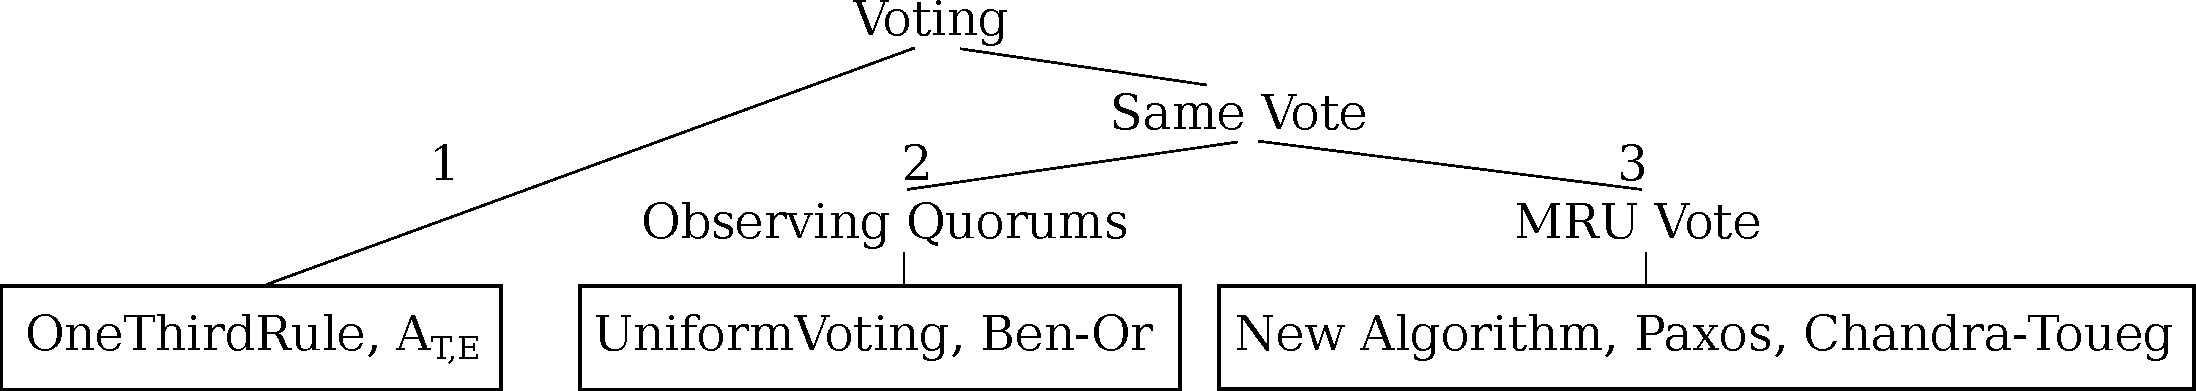
\includegraphics[scale=0.35]{ref-tree}
  \caption{The consensus family tree. Boxes contain models of concrete algorithms.}
  \label{fig:consensus-tree}
\end{figure*}

Figure~\ref{fig:consensus-tree} shows the resulting refinement tree
for our development. It captures the relationships between the
different consensus algorithms found at its leaves: OneThirdRule,
$A_{T,E}$, Ben-Or's algorithm, UniformVoting, Paxos, Chandra-Toueg
algorithm and a new algorithm that we present. The refinement tree
provides a natural classification of these algorithms. The new
algorithm answers a question raised
in~\cite{charron-bost_heard-model:_2009}, asking whether there exists
a leaderless consensus algorithm that requires no waiting to provide
safety, while tolerating up to $\frac{N}{2}$ process failures.

Our abstract (non-leaf) models are represented using unlabeled
transition systems. For the models of the concrete algorithms, we
adopt the Heard-Of model~\cite{charron-bost_heard-model:_2009}) and
reuse its Isabelle formalization by Debrat and
Merz~\cite{DBLP:journals/afp/DebratM12}. The Heard-Of model belongs to
a class of models we refer to as \emph{lockstep}, and which are
applicable to algorithms which operate in communication-closed
rounds. For this class of algorithms, the asynchronous setting is
replaced by what is an essentially a synchronous model weakened by
message loss (dual to strengthening the asynchronous model by failure
detectors). This provides the illusion that all the processes operate
in lockstep. Yet our results translate to the asynchronous setting of
the real world, thanks to the preservation result established
in~\cite{chaouch-saad_reduction_2009} (and formalized
in~\cite{DBLP:journals/afp/DebratM12}).

\section{Preliminaries}
\label{sec:introduction}

\input{session}  

\bibliographystyle{abbrv}
\bibliography{root}


\end{document}
